\documentclass[10pt,letterpaper]{article}
\RequirePackage{amsthm,amssymb,amsmath,graphicx}
\RequirePackage[top=2cm, bottom=2cm, left=2.5cm, right=3cm]{geometry}
\usepackage{caption}
\usepackage{subcaption}
\usepackage[pagebackref=false,colorlinks,linkcolor=black,citecolor=magenta]{hyperref}
\RequirePackage{MnSymbol}
\newcommand{\eqn}[2]{
\begin{equation}
\begin{split}
#1
\label{#2}
\end{split}
\end{equation}
}
%%%%%%%%%%%%%

%       \eqn{
%       x=x^2
%       }{label}

%%%%%%%%%%%%%
\newcommand{\feqn}[2]{
\begin{tcolorbox}[width=7in, colback=white]
\begin{equation}
\begin{split}
#1
\label{#2}
\end{split}
\end{equation}
\end{tcolorbox}
}
%%%%%%%%%%%%%%%
\newcommand{\hl}{
\begin{center}
\line(1,0){450}
\end{center}}
\setlength{\parindent}{0pt}
%\settextfont{B Nazanin}
\usepackage{lipsum}
\begin{document}
\Large
\begin{center}
The assignment \#5 of the \textbf{ComNet} course
\end{center}
\hl
Q1)

a. Why routing is first required to be settled before being able to perform forwarding?

b. What are ``layer 3 switches'' and which layer of protocol stack is being implemented in them?
\newline
\newline
Q2) 
\begin{table}[h]
\begin{center}
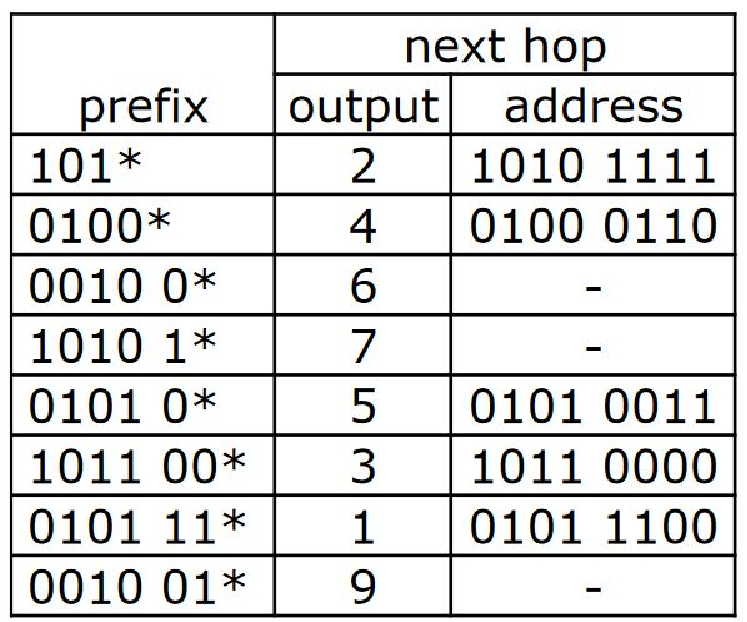
\includegraphics[width=60mm]{Table1}
\caption{Forwarding table}
\end{center}
\end{table}
Table 1 represents a forwarding table for an IP router (for simplicity, we are using 8 bit addresses).

(a) If a packet arrives with destination address 1010 0110, what output is it sent to, and what is the IP address of the next network-level component to receive the packet?

(b) If a packet arrives with destination address 0010 0110, what output is it sent to, and what is the IP address of the next network-level component to receive the packet?

(c) If a packet arrives with destination address 1011 0010, what output is it sent to, and what is the 
IP address of the next network-level component to receive the packet?
\newline
\newline
Q3) A router has $5$ input links and $5$ output links. The probability that a packet may come to an input link in a full time slot is $0.5$, where the incoming rate at that input link becomes $R$. Also assume that no two packets are headed for an output interface.

a) what, in the worst case, must the minimum rate of the switch fabric be  to avoid HOL blocking?

b) if the rate of the switch fabric is $3R$, and all the incoming packets are assumed to arrive simultaneously, what is the total average delay of HOL blocking for the blocked packets?
\newline
\newline
Q4) Consider a router that interconnects three subnets: Subnet 1, Subnet 2, and Subnet 3. Suppose all of the interfaces in each of these three subnets are required to have the prefix 223.1.17/24. Also suppose that Subnet 1 is required to support at least 60 interfaces, Subnet 2 is to support at least 90 interfaces, and Subnet 3 is to support at least 12 interfaces. Provide three network addresses (of the form a.b.c.d/x) that satisfy these constraints.
\newline
\newline
Q5) Assume the \textbf{Random Early Detection} algorithm is used for maintaining the input buffer of the input interfaces.
In brief this algorithm works as follow: The packets arrive with probability $p$ to each input interface at each timeslot. The packets have a constant length of $L$. The minimum and maximum thresholds are set to $5L$ and $8L$, respectively such that if the length of the queue falls within these thresholds, the new incoming packets are dropped with probability $1\over 5$. If the length of the queue becomes $8L$ or more, the new incoming packets are dropped with probability $1$. 

What is the probability that a newly-arrived packet is dropped?

(Hint: a queue is defined by a consecutive array of packets with no empty room between them. For further information about the Random Early Detection algorithm, you can check section 4.3.4, ``Where Does Queuing Occur?'', page 329 of ``Computer Networking; A top down approach'').
\end{document}